\cotefile{131}
\scanpage{2}
\mspage{A}
\margin{\unsure{conditions} \unsure{d'exactitude}}
\margin{\figure{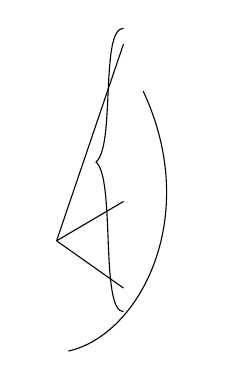
\begin{tikzpicture}[x=1cm,y=1cm]
\draw (1,3.6) .. controls (.7,3.6) and (.9,2.1) .. (.65,1.9) .. controls (.9,1.7) and (.7,0) .. (1,0);
\draw (.15,.9)--(1,3.4) (.15,.9)--(1,1.4) (.15,.9)--(1,.3);
\node at (-.1,.3) {$\varprojlim$};
\draw (1.25,2.8) .. controls (2,1.2) and (1.2,-.3) .. (.3,-.5);
\node at (0,-.5) {$\varinjlim$};
\end{tikzpicture}}}

$1^\circ$ $F$ faisceau pour la top \unsure{fppc|fpqc}
\margin{$\left\{\begin{array}{l}
\text{a) de nature locale Zariski}\\
\text{b) compatible aux \unsure{changts} \unsure{fid.}}\\
\text{\unsure{plt} \unsure{par.} \unsure{qcts} affines}
\end{array}\right.$}

$2^\circ$ $F$ commute aux $\varinjlim$ d'anneaux
\margin{(propriété \uline{relative})}

$3^\circ$ $F$ commute aux $\varprojlim$ adiques d'anneaux \uuline{\uline{artiniens}}

$4^\circ$ Pour tout anneau artinien $A$ sur $S$, $F_{\unsure{A}}$ est exact à \unsure{g.} sur la catégorie des \unsure{algèbres} \deleted{artiniens} finies sur $A$ (ou aussi, une suite exacte
\[
 A\longrightarrow A'\rightrightarrows A'\otimes_A A'=A''
\]
\inserted{$A$ artinien local}
\deleted{d'anneaux artiniens}, avec $A'\deleted{A''}$ \unsure{finis} sur $A$,
\inserted{[ext. résiduelle triviale, $\operatorname{long}_A A'/A=1$]}
donne une suite exacte
\[
 F(A)\mathrel{\unsure{-|\longrightarrow}}F(A')\rightrightarrows F(A'')
\]
].

\margin{\uline{finitude} \uline{ou} \uline{discrétion}}
\margin{\unsure{pour} \unsure{assurer|aux} \unsure{foncteurs} \unsure{sur} $X/k$\quad
$F(k)\xrightarrow{\sim}F(X)$ \unsure{pour} \unsure{v.} \unsure{(de t.f. sur k)}\quad
\unsure{n'induit aucune} \unsure{f.}\quad (\unsure{ou :} $X$ intègre)}
$5^\circ$ \deleted{\unsure{F séparé}} Pour tout anneau \deleted{\unsure{local}} \deleted{\unsure{complet}} \inserted{corps alg clos} $K$ sur $S$, et $\forall\ \xi\in F(K)$, l'anneau $B$ sur $K$ qui proreprésente $F_K$ en $\xi$ est \uline{fini} sur $K$.
\margin{(propriété \uline{relative})}

\margin{\uline{séparation}}
$6^\circ$ $F$ est \uline{séparé} sur $S$
\inserted{(par critère valuatif)}
\margin{(propriété \uline{relative})}

\margin{critère de \uline{modularité}\quad a) \uline{locale}}
$7^\circ$ Pour tout $S'$ local noeth complet, \inserted{sur $S$} $\forall\ t\longrightarrow Z$ \inserted{local} fini sur $S$, pt fermé $t$, \deleted{\unsure{a}}
\unsure{tout} $\unsure{\eta|y}:Z\longrightarrow F_{S'}$ [$\simeq\unsure{\eta|y}\in Z\mathrel{\unsure{-|\longrightarrow}}F$]
qui est \unsure{modulaire} (pour $F_{S'}$) au pt fermé $t$ de $Z$, $\unsure{\eta|y}$ est \unsure{modulaire} \inserted{[ou tout au moins, étale]} en tout point.
\diagram{\begin{tikzcd}
F\arrow[d] & F_{S'}\arrow[l]\arrow[d] & \\
S\arrow[r,no head] & S' & Z\arrow[l]\arrow[ul,"\unsure{\eta|y}"']
\end{tikzcd}}
\margin{On peut supposer $S'$ \unsure{irréductiblement} de dim $1$ (et $\unsure{F_{s'_0}|F_{s'}}$ représentable, \unsure{si} \deleted{\unsure{sur} $S'$} $s'$ est le pt générique de $S'$)}

\margin{b) \uline{générique}}
$8^\circ$ Pour tout $S'$ noeth irréductible sur $S$, et $Z\mathrel{\unsure{\longrightarrow|-}}S'$ \inserted{irréductible} \uline{fini} sur $S'$, $\unsure{\eta|y}:Z\longrightarrow F_{S'}$ tel que $\unsure{\eta|y}$ soit \unsure{modulaire} pour $F_{S'}$ au pt générique $z$ de $Z$, il existe un ouvert $U\ni z$ tel que $\unsure{\eta|y}$ soit \unsure{modulaire} (ou tt au moins étale) en tt point de $U$
\mspage{1}
\scanpage{3}
Dans le cas du critère pour les foncteurs non ramifiés, remplacer $5^\circ$ par la non ramification \inserted{(en artinien)}, et bloquer $4^\circ$ et $5^\circ$ en une condition unique aussi simple que possible [\unsure{Caractérisation} des foncteurs proreprésentables \uline{non ramifiés}]
\mspage{2}
\scanpage{4}
On notera que les conditions $1^\circ$ à $8^\circ$ sont stables par tte extension de la base. Sauf $2^\circ$, $5^\circ$, $6^\circ$, ce sont des conditions \uline{absolues} sur $F$.

Pour prouver la représentabilité de $F$, on commencera par le faire pour $n=\dim S<+\infty$, \deleted{\unsure{en suppos}}

\textcircled{1} $\dim S=0$. On est ramené au cas $S$ local artinien, on construit un préschém. loc. qu. fini sur $S$ grâce à \textcircled{$4^\circ$}, \textcircled{$5^\circ$}, on voit qu'il représente $F$ grâce à \textcircled{$1^\circ$}a, \textcircled{$2^\circ$}, \textcircled{$3^\circ$} [cf. notes jointes, cor $2$ à prop. $1$] OK. \uline{NB} On n'a eu besoin que de $1^\circ$ à $5^\circ$

\textcircled{2} $\dim S=n>0$, $S$ \uline{local complet}. Soit $s$ son pt fermé, \deleted{\unsure{---}} et $U=S-s$, alors par l'hypothèse de récurrence [où \textcircled{$1^\circ$} : \textcircled{$5^\circ$} suffisent si $S$ de dim $1$] on sait que $F_U$ est représentable \inserted{par un $X_U$}. De plus, grâce à \textcircled{$\unsure{4^\circ|2^\circ}$}, \textcircled{$5^\circ$}, on construit une famille de schémas \uline{finis} $X_i$ sur $S$, \inserted{(utilisant $S$ complet)} \unsure{correspondants} aux pts de $F_0$, et \deleted{grâce à} grâce à \textcircled{$3^\circ$} des hom $u_i:X_i\longrightarrow F$. En vertu de la prop. $2$ des notes, on est ramené à vérifier que $u_{iU}:X_{iU}$\inserted{$\longrightarrow X_U$} \uline{immersions} \uline{ouvertes}, à images deux à deux disjointes. Ce dernier fait provient de l'\uline{hypothèse}
\margin{\uline{N.B.} Si $\dim S=1$, $S$ local (\unsure{compl.}), l'hypothèse $8^\circ$ est inutile.}
\mspage{3}
\scanpage{5}
\textcircled{$6^\circ$}. Utilisant la condition \textcircled{$7^\circ$}, on est ramené à montrer que $X_i\xrightarrow{u_i}F$ est modulaire en le centre $x_i$ de $X_i$. Comme la restriction $u_0:X_0\mathrel{\unsure{-|\longrightarrow}}F_0$ est modulaire (donc \deleted{\unsure{le}} $k(x_i)$ est un corps de définition pour $u_i:k(x_i)\longrightarrow F$ sur $S$] il reste à vérifier la condition modulaire. Nous allons \deleted{\unsure{commencer}} d'abord démontrer le théorème dans le cas où la condition $7^\circ$ est remplie, en y exigeant seulement $\unsure{\eta|y}$ \uline{pro-modulaire} \inserted{sur $S$} en $z$. De plus, $X$ est loc. qu. fini sur $S$ par construction, et séparé sur $S$ par $6^\circ$.
\margin{Dégager un lemme à cet effet}
\margin{Pour l'instant on n'utilise \deleted{\unsure{pas}} \inserted{\unsure{que la}} \deleted{\unsure{la plus}} \inserted{\unsure{forme}} \unsure{affaiblie} \deleted{\unsure{nouvelle}} de $7^\circ$}

\textcircled{3} $\dim S=n>0$, $S$ local. On sait par $2)$ que $F_{\hat S}$ est représentable par un $X_{\unsure{\hat S}}$ \inserted{loc.} quasi-fini, et séparé sur $S$. Il en résulte que la donnée de descente \unsure{canon.} sur $F_{\hat S}$ est effective, \deleted{Utilisant} d'où un $X$ sur $S$, \inserted{loc.} quasi-fini sur $S$ et séparé sur $S$.

Utilisant $1^\circ$, b) on trouve qu'il représente $F$.

\textcircled{4} $\dim S=n$, $S$ quelconque. \deleted{\unsure{Comme le}} On utilise le

\uline{Lemme} \inserted{$F$ comme dessus.} Supposons que pour $\forall\ a\in S$, $F_{S^a}$ sur $S^a=\operatorname{Spec}\mathcal O_{S,a}$ soit représentable. Alors $F$ est représentable.
\margin{\figure{\begin{tikzpicture}\draw (0,0)--(0,1.4);\end{tikzpicture}}}

On utilise la prop $3$ des notes jointes.
\mspage{4}
\scanpage{6}
Compte tenu des conditions $1^\circ$ et $2^\circ$, on est ramené à vérifier la condition de constructibilité de loc. cit.
\mspage{5}
\scanpage{7}
$C_1$ peut aussi se mettre sous la forme

$7^\circ)$ Pour $\forall\ S'\longrightarrow S$ [avec $S'$ \deleted{local} noeth. \inserted{[local]} complet [irréduct. de dim $1$] et $S'_0$ sous-\deleted{\unsure{pré}}schéma défini par un idéal nilpotent [de carré nul], \deleted{toute} ouvert $U\subset S'$ \inserted{d'adhérence schématique $S'$} [$U=S'-\text{pt fermé}$], et \deleted{section de $F_T$} $S'$-morphisme $\unsure{\eta|y}_0:S'_0\mathrel{\unsure{-|\longrightarrow}}F_{S'}$, \deleted{\unsure{tel que et}} \deleted{$\unsure{\eta|y}:S'$} si $\unsure{\eta|y}_0|U_0$ se prolonge en $\unsure{\eta|y}_{\unsure{U}}:U\mathrel{\unsure{-|\longrightarrow}}F_{S'}$, alors $\unsure{\eta|y}_0$ se prolonge en $\unsure{\eta|y}:S'\mathrel{\unsure{-|\longrightarrow}}F_{S'}$.
\margin{\figure{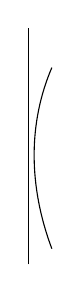
\begin{tikzpicture}\draw (0,0)--(0,3);\draw (.3,.2)..controls (0,1) and (0,1.8)..(.3,2.5);\end{tikzpicture}}}

[\uline{NB} Cette condition est \uline{vide} si $F\longrightarrow S$ est étale]

\margin{Cela se met sous la forme :}
\margin{\deleted{\illegible{1}}}
$8^\circ)$ Soit $S'$ sur $S$ noeth irréductible, \inserted{de pt gén. $x$} $S'_0$ défini par un idéal \deleted{nilpotent}, $\unsure{\eta|y}:S'_0\longrightarrow F_{S'}$, supposons que $\unsure{\eta|y}$ soit modulaire \inserted{(i.e. étale)} en $x$, alors il est modulaire au voisinage de $x$.

\figure{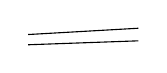
\begin{tikzpicture}\draw (0,0)--(1.4,.08);\draw (0,-.13)--(1.4,-.08);\end{tikzpicture}}

Revenons au cas général, \inserted{(pas néc. non ram.)} je dis que (A) et (B) peuvent se remplacer par

\margin{(D)}
$(D_1)$ Si $S'$ noeth sur $S$, $\unsure{X|Z}$ \deleted{\unsure{qu. fini}} sur $S'$, et $\unsure{\eta|y}:\unsure{X|Z}\longrightarrow F_{S'}$ un $S'$-morphisme, l'ens des pts où $\unsure{\eta|y}$ est inf\textsuperscript{t} étale est \uline{ouvert} ; \deleted{Et}
\margin{\figure{\begin{tikzpicture}\draw (0,0)--(0,1.6);\end{tikzpicture}}}
\deleted{[Conditions analogues pour}
\diagram{\begin{tikzcd}\deleted{F}\arrow[r,"\deleted{\mathrm{diag}}"]&\deleted{F\times_S F}\end{tikzcd}}
\deleted{, puis $\forall$ \unsure{changement} de base, \unsure{pour} $\unsure{\eta|y}$ \unsure{capturant} \unsure{l'expression} \unsure{des} $7^\circ$ et $8^\circ$]}
\deleted{\unsure{et} \unsure{sur} \uline{\unsure{un}} voisinage)}
\deleted{il en est de même \unsure{pour} le \unsure{foncteur} $X\times_{F_{S'}}X$ sur $S'$, \unsure{pour} \unsure{le} \unsure{morphisme}}
\diagram{\begin{tikzcd}\deleted{\unsure{X\times_{S'}X|X_{S'}}}\arrow[r]&\deleted{\unsure{S'}}\end{tikzcd}}
\deleted{\unsure{pour} $\unsure{T}$ \unsure{plongé} dans $X\times_S X$, de sorte que \unsure{cette} condition s'exprime au moyen de $7^\circ$ et $8^\circ$].}
\mspage{6}
\scanpage{8}
\mspage{7}
\begin{center}4 - 27 -\end{center}
\margin{n\textsuperscript{o} 392}

Soit maintenant $L_1$ un second sous-module libre de $M$, de rang $n$. Puisque $S^{-1}L=S^{-1}L_1$, il existe $s\in S$ tel que $sL_1\subset L$ ; on peut donc se borner à prouver que si $L_1\subset L_2$ sont deux sous-modules libres de $M$, on a $c(\chi(M/L_1))=c(\chi(M/L_2))$. Or, on a $\chi(M/L_1)=\chi(M/L_2)+\chi(L_2/L_1)$, et il résulte du n\textsuperscript{o} $6$, cor. de la prop. $14$, que $\chi(L_2/L_1)$ est un diviseur principal, donc $c(\chi(L_2/L_1))=0$. C. Q. F. D.

L'élément $c(\chi(M/L))$ sera noté $-c(M)$ dans ce qui suit ; nous dirons que $c(M)$ est la \uline{classe de diviseurs attachée à} $M$.

PROPOSITION 16.- (i) \uline{Soit} $0\longrightarrow M_1\xrightarrow{f}M_2\xrightarrow{g}M_3\longrightarrow0$ \uline{une suite exacte de} $A$-\uline{modules de type fini}. \uline{On a} :
\[
 c(M_2)=c(M_1)+c(M_3).
\]

(ii) \uline{S'il existe un pseudo-isomorphisme de} $M_1$ \uline{dans} $M_2$, \uline{on a} $c(M_1)=c(M_2)$.

(iii) \uline{Si} $T$ \uline{est un module de torsion}, \uline{on a} $c(T)=-c(\chi(T))$.

(iv) \uline{Si} $\underline a$ $\ne0$ \uline{est un idéal fractionnaire de} $K$, \uline{on a} $c(\underline a)=c(\operatorname{div}(\underline a))$.

(v) \uline{Si} $L$ \uline{est un} $A$-\uline{module libre}, \uline{on a} $c(L)=0$.

Pour prouver (i), considérons un sous-module libre $L_1$ (resp. $L_3$), de $M_1$, (resp. $M_3$), tel que $M_1/L_1$, (resp. $M_3/L_3$), soit un module de torsion. Puisque $L_3$ est libre et $g$ surjectif, il existe dans $g^{-1}(L_3)$ un supplémentaire libre $L_{23}$ de $\operatorname{Ker}(g)$, isomorphe à $L_3$, (\uline{Alg.}, chap. II, 3e éd., \S\ $1$, n\textsuperscript{o} $11$, prop. $21$) ; mais $\operatorname{Ker}(g)=f(M_1)$ contient $f(L_1)=L_{12}$ qui est libre puisque $f$ est injectif. La somme $L_2=L_{12}+L_{23}$ est directe, et $L_2$ est donc un sous-module \uline{libre} de $M_2$. On a en outre le diagramme commutatif :
\diagram{\begin{tikzcd}
0\arrow[r]&L_1\arrow[r]\arrow[d]&L_2\arrow[r]\arrow[d]&L_3\arrow[r]\arrow[d]&0\\
0\arrow[r]&M_1\arrow[r,"f"']&M_2\arrow[r,"g"']&M_3\arrow[r]&0
\end{tikzcd}}
\scanpage{9}
\uline{Axiomes} $1^\circ:6^\circ$, et.

A) Si $S'$ local noeth complet, \inserted{[de dim $1$ si on veut]} la promodularité de
\[
 \unsure{X|Z}\xrightarrow{\unsure{\eta|y}}F_{S'}
\]
en $z$ sur le pt fermé de $S'$ ($\unsure{X|Z}$ fini sur $S'$) implique $\unsure{\eta|y}$ \deleted{modulaire} imm. ouverte (et on peut supposer $F|(S'-\{s'\})$ repr.)

B) \deleted{Si \unsure{aux des}} $S'$ noeth sur $S$, $\unsure{X|Z}$ sur $S$, $\unsure{\eta|y}:\unsure{X|Z}\mathrel{\unsure{-|\longrightarrow}}F_{S'}$, et $x\in X$ sont tels que $\unsure{\eta|y}$ \unsure{modulaire} en $x$, alors $\exists\ U\ni x$ voisinage ouvert, t.q. $\unsure{\eta|y}|U:U\mathrel{\unsure{-|\longrightarrow}}F_{S'}$ soit une imm. ouverte [On \unsure{peut|pt} $\unsure{\simeq|\text{même}}$ supposer que $X\times_{S'}\mathcal O_{S',s'}\longrightarrow F_{\operatorname{Spec}\mathcal O_{S',s'}}$ est une imm. ouverte]

\uuline{Cas particuliers}

\deleted{(i) \illegible{1} $F\longrightarrow S$ un \uline{monomorphisme}. Alors (A) et (B) sont contenus dans}

\deleted{(C) Pour $\forall\ S'$ noethérien$/S$, \unsure{lisse}}
\inserted{$X\longrightarrow S'$ un \deleted{\unsure{mor.}} \unsure{mor.}}
\deleted{et $\unsure{\eta|y}:X\mathrel{\unsure{-|\longrightarrow}}F_{S'}$, l'ens des $x\in X$ en lesquels $\unsure{\eta|y}$ est \inserted{inf.} étale est ouvert.}

\margin{\uuline{Lemme}\quad On peut supposer en A resp. B que $X\longrightarrow S'$ une \uuline{imm.} \uline{fermée}.}
\margin{définie \unsure{si} on veut par un idéal de carré nul}

Si $F\mathrel{\unsure{-|\longrightarrow}}S$ \uline{non ramifié}, les conditions (A) et (B), sont \inserted{alors} contenues dans

(C) Si $S'$ noeth. sur $S$, \deleted{$S'_0$} \inserted{$S'$ \uline{imm. fermée}, définie par un idéal de carré nul} \deleted{\unsure{tf.}} sur $S'$, $\unsure{\eta|y}:X\mathrel{\unsure{-|\longrightarrow}}F_{S'}$, l'ens \inserted{$U$} des pts en lesquels $\unsure{\eta|y}$ est \uline{inf\textsuperscript{t}.} \uline{étale} est \uline{ouvert} i.e.

$(C_1)$ stable par générisation [est \deleted{\unsure{un}} équivalent à A]

$(C_2)$ si $x\in U$, alors \deleted{l'ens} $U\cap\bar x$ est un voisinage de $x$ dans $\bar x$.
\margin{\figure{\begin{tikzpicture}\draw (0,2)--(0,3);\draw (0,0)--(0,.5);\end{tikzpicture}}}

\uline{N.B.} La condition $(C_1)$ est automatique si $F\longrightarrow S$ est \uline{étale}
\mspage{8}
\scanpage{10}
\mspage{9}
\begin{center}4 - 26 -\end{center}
\margin{n\textsuperscript{o} 392}
\[
 (8)\qquad \chi(\operatorname{Coker}(f))=\operatorname{div}(\det(\underline{U})).
\]
On peut considérer $L_1$ et $L_2$ comme des réseaux dans $V_1=L_1\otimes_A K$ et $V_2=L_2\otimes_A K$ respectivement, $f$ s'étendant en un $K$-homomorphisme $f_{(K)}:V_1\longrightarrow V_2$. On a alors $(\operatorname{Coker}(f))_{(K)}=\operatorname{Coker}(f_{(K)})$ et dire que $\operatorname{Coker}(f)$ est un $A$-module de torsion signifie que $\operatorname{Coker}(f_{(K)})=0$ ; or, il revient au même de dire que $f_{(K)}$ est surjectif ou que $\det(\underline{U})\ne0$, d'où la première assertion. D'autre part, on peut écrire $f(L_1)=u(L_2)$, où $u$ est un endomorphisme de $L_2$ de déterminant $\det(\underline{U})$ ; comme $\operatorname{Coker}(f)=L_2/u(L_2)$, la formule (8) résulte de (7) et (6).

\uline{Exemple}.- Si $A=Z$, le groupe des diviseurs de $A$ s'identifie au groupe multiplicatif $Q_+^*$ des nombres rationnels $>0$. Pour tout groupe commutatif fini $T$, $\chi(T)$ est l'\uline{ordre} de $T$ ; le corollaire précédent montre que l'ordre du groupe $\operatorname{Coker}(f)$ est égal à la \uline{valeur absolue} de $\det(\underline{U})$.

7. \uline{Classes de diviseurs attachéesaux modules de type fini}.

Les notations et hypothèses sont celles des n\textsuperscript{os} $2$ à $6$. Rappelons que l'on note $C(A)$, (ou simplement $C$), le \uline{groupe des classes de diviseurs} de $A$, quotient de $D(A)$ par le sous-groupe des diviseurs principaux. Pour tout diviseur $d\in D$, nous noterons $c(d)$ sa classe dans $C$.

PROPOSITION 15.- \uline{Soit} $M$ \uline{un} $A$-\uline{module de type fini}. \uline{Il existe un sous-module libre} $L$ \uline{de} $M$ \uline{tel que} $M/L$ \uline{soit un module de torsion}, \uline{et l'élément} $c(\chi(M/L))$ \uline{de} $C$ \uline{ne dépend pas du sous-module libre} $L$ \uline{choisi}.

Posons $S=\unsure{A-\{0\}|A:-\{0\}}$, et soit $V=S^{-1}M=M\otimes_A K$ ; si $n$ est la dimension de $V$ sur $K$, il existe $n$ éléments $e_i$, $(1\le i\le n)$, de $M$ dont les images canoniques dans $V$ forment une base de $V$ ; ces éléments sont évidemment linéairement indépendants dans $M$, donc engendrent un sous-module libre $L$ de $M$ tel que $S^{-1}(M/L)=S^{-1}M/S^{-1}L=0$, de sorte que $M/L$ est un module de torsion.
\scanpage{12}

\textcircled{\unsure{10|9}°} Si $T$ noeth. \unsure{irred.} sur $S$, $\exists U\subset T$ ouvert non vide tel que $F_U$ soit représentable.
\margin{peut se formuler de façon un \unsure{peu plus} faible, avec impossibilité \unsure{générique} de prolonger}

\textcircled{1°} Foncteur $F$ de nature locale

\textcircled{2°} $F$ compatible avec descente fid plt qu. \unsure{cpte}
\margin{\uuline{localité}}

\textcircled{3°} $F$ commute aux $\varinjlim$ d'anneaux

\textcircled{4°} $F$ commute aux $\varprojlim$ d'anneaux \inserted{Artiniens} sous les conditions habituelles

\textcircled{\unsure{7|5}°} $F$ ``non ramifié'' \deleted{\unsure{et}} (Il suffit: sur les artiniens)
\inserted{et \unsure{$=$|m\textsuperscript{e}}: sur les $k[T]/(t^2)$}

\deleted{6° Tout pt de $F$ à valeurs dans une \deleted{corps} \inserted{extension} $K$ d'un $k(s)$, provient d'une sous-extension finie}

\textcircled{\unsure{5|7}°} $F$ proreprésentable universellement,
\figure{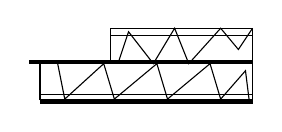
\begin{tikzpicture}[x=.45cm,y=.45cm]
\draw (0,0)--(6,0)--(6,2)--(2,2)--(2,1)--(0,1)--cycle;
\draw[line width=1.2pt] (-.3,1.05)--(6,1.05) (0,-.08)--(6,-.08);
\draw (0.5,1)--(.7,0)--(1.8,1)--(2.1,0)--(3.3,1)--(3.6,0)--(4.8,1)--(5.1,0)--(5.8,.8)--(5.9,0);
\draw (2.2,1)--(2.5,1.9)--(3.2,1)--(3.8,2)--(4.2,1)--(5.1,2)--(5.6,1.4)--(6,2);
\draw (0,.12)--(6,.12) (2,1.8)--(6,1.8);
\end{tikzpicture}}

\textcircled{8°}: $F$ ``séparé'' (critère valuatif).

\textcircled{9°} Pour tt $A$ anneau local noeth \inserted{complet} de dim 1, irréductible, sur $S$, et $\forall$ idéal $I$ de $A$ nilpotent, \inserted{i.e. $\unsure{\mathfrak p}$ idéal \unsure{premier|primaire}} \deleted{\unsure{$\xi$}} $\unsure{\xi_0|\eta_0}\in F(A/I)$, \deleted{\unsure{si $\unsure{\xi_0|\eta_0}\in\operatorname{Im}F(A_{\unsure{\mathfrak p|\eta}})$}} \deleted{\unsure{se prolonge en un $\unsure{\eta|y}\in F(A/\unsure{I^n})$,}} \deleted{\unsure{alors $\xi\in\varprojlim(A/\unsure{I^n})$}} \deleted{\unsure{provenant d'un} \illegible{1} \unsure{pour} $\xi_0\in F(A_{\unsure{\mathfrak p|\eta}}/I_{\unsure{\mathfrak p|\eta}})$}
\margin{automatique dans le cas étale}

\margin{\uline{9°} Pour $\forall S'$ \inserted{\unsure{noeth. irred.}} sur $S$, muni d'un \deleted{\unsure{schéma}} \inserted{Idéal} $I$ de carré nul [si on veut, \unsure{annulé par le nilradical}], définissant $S'_0=V(I)$, et $\forall\unsure{\eta|y}_0:\deleted{\unsure{S'_0}}\inserted{S'_0\to F_{S'}}$ ($S'$-linéaire), qui ne se prolonge pas au pt. gén. $\unsure{\eta|y}$ à un plus-\unsure{petit|grand} sous-schéma de $S'_{\unsure{\eta|y}}$ que $S'_{0\unsure{\eta|y}}$, il existe un voisinage ouvert $U$ de $\unsure{\eta|y}$, tel que pour tt $s\in S'$, $\unsure{\eta|y}|S'^s_0$ ne se prolonge pas à un plus grand sous-schéma de $S'^s$.
\diagram{\begin{tikzcd} F_{S'}\arrow[d,no head] & \\ S'\arrow[r,no head] & S'_0 \end{tikzcd}}
\deleted{\diagram{\begin{tikzcd} S' & \unsure{X}\arrow[l] \end{tikzcd}}}
\textcircled{A bis}}

\margin{N.B. \uline{8° et 9°} peuvent se remplacer par une condition unique, \unsure{faisant intervenir la|formulant la} \unsure{représentabilité} \unsure{non} dans la \unsure{formulation}, \unsure{en disant que une condition} \unsure{Modulaire ou} \unsure{pro-modulaire}, \deleted{$\unsure{F}$} \unsure{commute à l'extension} (\unsure{fid. plt}) de la base}

\margin{\deleted{peut se remplacer \uline{par}: si $A\to A'$ est injectif, $A'$ fini sur $A$, \deleted{\unsure{fid plt sur}} $A$ artinien \inserted{local}, \deleted{\unsure{alors $F(A)\xrightarrow{\sim}F(A')$}} [ext. résiduelle triviale, \deleted{\unsure{longueur}} $\operatorname{long}_A A'/A=1$] alors $F(A)\xrightarrow{\sim}F(A')$}}

\diagram{\begin{tikzcd}[column sep=large,row sep=large]
\unsure{7}^\circ\arrow[ddr,bend right=35] & \\
\text{peut se remplacer par}\arrow[r] & \unsure{5}^\circ \\
&9^\circ\arrow[dll,bend left=15]\\
\text{automatique dans le cas étale} &&
\end{tikzcd}}
\mspage{11}
\scanpage{13}
\begin{center}-- 54 --\end{center}
\hfill n° 371

\[
(17)\qquad \varepsilon(\alpha,\beta)=\prod_{i>j}\varepsilon_{ij}(\alpha_i,\beta_j).
\]

En effet, le second membre de (16) appartient évidemment à $E_{\alpha+\beta}$ et l'application $(x_1,\ldots,x_n,y_1,\ldots,y_n)\longrightarrow\varepsilon(\alpha,\beta)\bigotimes_{i\in I}(x_i y_i)$ est $A$-multilinéaire dans le produit des $E_{\alpha_i}$ et des $E_{\beta_j}$ $(1\leq i\leq n,\ 1\leq j\leq n)$. Il s'agit ensuite de prouver que la multiplication ainsi définie sur $E$ est \uline{associative}; or, si $\gamma=(\gamma_i)$ est un troisième élément de $\Delta$, et $z_i\in E_{i,\gamma_i}$ pour $1\leq i\leq n$, on a
\[
\begin{aligned}
((\bigotimes_i x_i)(\bigotimes_i y_i))(\bigotimes_i z_i)&=\varepsilon(\alpha+\beta,\gamma)\varepsilon(\alpha,\beta)\bigotimes_i(x_i y_i z_i)\\
(\bigotimes_i x_i)((\bigotimes_i y_i)(\bigotimes_i z_i))&=\varepsilon(\alpha,\beta+\gamma)\varepsilon(\beta,\gamma)\bigotimes_i(x_i y_i z_i)
\end{aligned}
\]
et tout revient donc à vérifier l'identité
\[
\varepsilon(\alpha+\beta,\gamma)\varepsilon(\alpha,\beta)=\varepsilon(\alpha,\beta+\gamma)\varepsilon(\beta,\gamma)
\]
qui résulte aussitôt des relations
\[
\begin{aligned}
\varepsilon(\alpha+\beta,\gamma)&=\varepsilon(\alpha,\gamma)\varepsilon(\beta,\gamma)\\
\varepsilon(\alpha,\beta+\gamma)&=\varepsilon(\alpha,\beta)\varepsilon(\alpha,\gamma)
\end{aligned}
\]
elles-mêmes conséquences immédiates de la définition (17).

Si $e_i$ désigne l'élément unité de $E_i$, on sait que $e_i$ est homogène de degré 0, donc $e=\bigotimes_{i\in I}e_i$ est homogène de degré 0, et il résulte de (16) et des relations $\varepsilon_{ij}(\alpha_i,0)=\varepsilon_{ij}(0,\beta_j)=1$ que $e$ est élément unité de $E$, ce qui achève de définir sur $E$ la structure de $A$-algèbre graduée cherchée. On prendra ensuite $h_i(x_i)=x_i\otimes\bigotimes_{j\ne i}e_j$; il résulte de (16) que $h_i$ est un homomorphisme d'algèbres et vérifie les conditions 1° et 2° de l'énoncé, en vertu des relations $\varepsilon_{ij}(0,\beta_j)=\varepsilon_{ij}(\alpha_i,0)=1$. Ces mêmes relations prouvent que l'on a
\[
(18)\qquad \bigotimes_{i\in I}=\prod_{i\in I}h_i(x_i)
\]
où le second membre est le produit de la \uline{séquence} $(h_i(x_i))_{i\in I}$ pour la structure
\mspage{12}
\scanpage{14}
\uline{Théorème} Soit $S$ préschéma loc. noeth, $F:(\mathrm{Sch})_{/S}^{\circ}\to\mathrm{Ens}$.

Pour que $F$ soit représentable par un $X$ \uline{localement quasi fini} sur $S$ et \uline{séparé} sur $S$, il \unsure{f|f\textsuperscript{t}} et \unsure{s|S} que $F$ satisfasse les conditions suivantes

1°) $F$ de nature locale

3°) $F$ ``commute aux $\varinjlim$ d'anneaux''

2°) $F$ compatible aux desc. fid. plts et qu. \unsure{cptes}
[Il le suffit pour $B\to\widehat B$, où $B$ est un anneau local \inserted{noeth} sur $S$] \deleted{\unsure{ess. de type fini et à ext. résiduelle finie}}

4°) $F$ commute aux $\varprojlim$ d'anneaux artiniens, pour $\widehat B=\varprojlim B_n$, avec $B$ comme dans 2°

5°) $F$ proreprésentable au dessus de \deleted{$\forall$ \unsure{les pts de} $S$}, \inserted{anneaux artiniens $A$ sur $S$} les anneaux $B$ qui \deleted{\unsure{re}}\inserted{pro}représentent $F$ en $A$ sont \uline{finis} sur \deleted{$\unsure{B}$}$A$ ]

6°) $F$ ``séparé'' (par critère valuatif\ldots)

\textcircled{7°} Pour \deleted{\unsure{tout}} $\forall A$ \deleted{comme dans 2°}, \inserted{anneau local noeth complet sur $S$}, et tout hom local $A\deleted{\unsure{\leftarrow}}\to B$, $B$ fini sur $A$, \deleted{et tt} $\unsure{\eta|y}\in F(B)$, \deleted{qui soit promodulaire}, \inserted{tel que $\unsure{\eta|y}$ soit modulaire,} [on verra que cel implique: pro-modulaire\ldots] et tout $\mathfrak p\in\operatorname{Spec}(B)$, $\unsure{\eta|y}_{\mathfrak p}\in F(B_{\mathfrak p})$ est modulaire. [Cf plus bas \unsure{des variantes|du contraire}, dans un cas particulier)
\margin{[en fait, \uuline{étale} suffit, \deleted{\unsure{et}} et cela signifie que $\unsure{\eta|y}:\operatorname{Spec}B\to F$ est étale]}

\textcircled{8°} [Pour $\forall$ \deleted{\unsure{tout}} schéma \deleted{\unsure{fini}} \inserted{noeth} irréductible $S'$ sur $S$, \deleted{pour} \inserted{et} $Z$ sur $S'$ muni de $\unsure{\eta|y}\in F(Z)=F_{S'}(Z)$, $z\in Z$ au dessus du pt gén. de $S'$, tel que $\unsure{\eta|y}$ soit modulaire

\margin{\uline{N.B.} On \unsure{fera résulter|peut vérifier} que les conditions 1° à 5°, [\unsure{et avec} 6°] $+$ 7° impliquent l'analogue de 7° sans hypo. de dim 1 ni \unsure{finitude}.}

\margin{Donner l'exemple-type ($S$ de dim 1) montrant que (8°) n'est pas surabondant, $\unsure{\simeq|=}$ si $F\Rightarrow$ non ramifié. Est-ce que 7° est surabondant? \uuline{Non}, si on \unsure{renforce aussi|remplace aussi} 4° au cas adique noeth. (pas artinien)}
\mspage{13}
\scanpage{15}
\figure{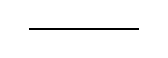
\begin{tikzpicture}\draw[line width=.8pt](0,0)--(1.4,0);\end{tikzpicture}}

\uline{Immersion ouverte}

Conditions \deleted{\unsure{1,2,3,4°}} \inserted{1°, 2°, 3°, 4°} et de plus

a) $F\to S$ est un \uline{monomorphisme} \uline{étale} pour les arguments artiniens.
\figure{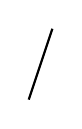
\begin{tikzpicture}\draw[line width=.8pt](0,0)--(.3,.9);\end{tikzpicture}}
\mspage{14}
\scanpage{16}
en $z$, il existe une partie ouverte \deleted{\unsure{de}} \inserted{non vide} $U$ de $Z$ telle que $z'\in U$ implique que $\unsure{\eta|y}$ est \deleted{étale en $z'$} modulaire en $z'$ [ou $=$ simplement \uline{étale} en $z'$]

\figure{\begin{tikzpicture}\draw[densely dotted](0,0)--(1.4,0);\end{tikzpicture}}

\uline{Corollaire 1} Pour que $F$ soit représentable par un $X$ \uline{étale} et \uline{séparé} sur $S$, il f et s qu'il satisfasse les conditions \deleted{1°) à 6°)} \inserted{1° 2° 3° 4° 6°}, et de plus

\deleted{\unsure{(Et)}} Le foncteur $F$ est étale (ou seulement, étale pour des arguments artiniens) \deleted{les $B$ de 5°) \unsure{sont} étales sur $A$}

\margin{\uline{Expliciter aussi le cas d'une immersion ouverte} [dont \unsure{le axiome|l'axiome} \unsure{direct|discret} est plus faible]}

\uline{Corollaire 2} Pour que $F$ soit représentable par un $X$ non ramifié et séparé sur $S$, il f. et s que les conditions 1°) à 6°), \deleted{\unsure{soient}} \inserted{ainsi que \textcircled{8°}} soient vérifiées, et de plus la condition \deleted{7} (NR.) \inserted{(qui implique 7°)}

\begin{enumerate}
\item[a)] Le foncteur $F$ est non ramifié (ou seulement, les $B$ dans 5°) sont non ramifiés sur $A$
\item[\textcircled{b}] Pour $\forall$ \deleted{\unsure{un point gén.}} \inserted{anneau local noeth} \deleted{$\unsure{A}$} \inserted{complet} de dim 1 \deleted{\unsure{d'un point de localité}} de $S$, \deleted{\unsure{avec $A$ premier}}, \inserted{irréductible}, d'idéal \deleted{et $\forall$ \unsure{$\eta\in$|$y\in$}} \inserted{premier minimal} $\mathfrak p$, et $\forall$ \deleted{$\unsure{\eta\in F|y\in F}$} \inserted{idéal} $I\subset\mathfrak p$, \inserted{tel que $I\mathfrak p=0$}, $\unsure{\eta|y}\in F(A/I)$, si $\unsure{\eta|y}_{\mathfrak p}\in\operatorname{Im}F(A_{\mathfrak p})$ alors $\unsure{\eta|y}\in\operatorname{Im}F(A)$.
\end{enumerate}

\margin{[Exprimer 8° ici par une impossibilité \uline{générique} de prolonger \ldots}

\uline{Remarque 3} La condition 8°) est conséquence de la \unsure{repré.} $\Rightarrow$ \unsure{Ce qu'il est néc.|Ce qui est néc.} pour que la conclusion soit \unsure{val. (loc.)}:
\mspage{15}
\scanpage{17}
\textcircled{RG} Pour $\forall S'$ \deleted{\illegible{2}} sous-préschéma fermé irréductible de $S$, $\exists$ ouvert non vide $U\subset S'$ tel que $F_U$ soit représentable par un préschéma loc de type fini sur $U$.

\uline{Remarque 4} \unsure{Limitation} des anneaux $A,B$ et schémas $S'\ldots$ qui devront être envisagés dans les conditions 2°, 4°, 5°, 7°, 8° \ldots

\uline{Exemples de foncteurs non ramifiés}

a) \unsure{Mémo-finité|Mono-finité}, plus généralement $G/H$, $H$ sous-groupe \uline{ouvert} $+$ \uline{fermé}, plat/$S$ \ldots

b) \deleted{\unsure{Champs de}} \inserted{Classes de} Correspondances divisorielles

c) Hom [pointés] dans un groupe commutatif

\unsure{d)} Hom de V.A. dans un groupe comm. [Hom de V.A.]

e) Immersions [qui s'introduisent p.ex. dans les pbs des \unsure{modules principaux} de divers \unsure{f\textsuperscript{rs}}, p.ex. des problèmes d'isomorphisme \ldots] en particulier \inserted{1°) morphismes diagonaux $F\to F\times_S F$ 2°) Foncteurs platificateurs}

d) Sous \deleted{groupes} schémas, \unsure{distingués|disjoints} d'un schéma en groupes \inserted{comm}
\diagram{\begin{tikzcd}[row sep=large] e)\\d)\arrow[u,bend left=80] \end{tikzcd}}

f) \uline{Décomposition} des fibres \inserted{\unsure{propres}} d'un morphisme en composantes connexes (\unsure{resp.} en composantes irred.).
[Les foncteurs obtenus ici sont même \uline{étales}]
Factorisations d'un morphisme fini \unsure{univ.} ouvert \ldots

\uline{Applications en vue.}

1) Un schéma abélien sur $S$ loc. noeth. normal est projectif sur $S$
[utiliser le schéma des correspondances divis. sur $X\times_S X$]

2) Existence du Picard d'un schéma propre sur un corps \deleted{[\unsure{Seshadri M.}} \inserted{[Chevalley--Seshadri--Grothendieck--Murre]}, plus généralement, sur une base $S$, existence au-dessus d'un ouvert non vide \ldots
\mspage{16}
\scanpage{18}
Façon d'exprimer
\mspage{17}
\scanpage{20}
En effet, \unsure{appliquant} ce qui est prouvé dans le cas non ramifié à l'étude de $F\mathbin{-}F\times_S F$, on trouve que c'est repr., et grâce à 6°, c'est une imm. fermée. Ceci posé, dans (A), $X\times_{F_{S'}}X$ est un sous préschéma fermé de $X\times_S X$, \inserted{fini sur $X$}, qui coïncide formellement avec la diagonale $X\hookrightarrow X\times_S X$, donc lui est identique; donc $X\mathbin{-}F$ est un \uline{monomorphisme}, d'autre part étant étale, c'est une imm. ouverte.

Dans $B$, on procède de façon analogue pour prouver $\exists U$ voisinage ouvert de $s$, tel que $\unsure{\eta|y}|(X|U))$ est un \uline{monomorphisme}; comme c'est \unsure{déjà fait} \unsure{pour|par} ``étale'', on gagne.
\mspage{19}
\scanpage{21}
\begin{center}4 -- 24 --\end{center}
\hfill n° 392

D'autre part, $(A:\underline a)_{\underline p}=A_{\underline p}:\underline a A_{\underline p}=\underline p^{-n_{\underline p}}A_{\underline p}$, donc $\ell_{\underline p}((A:\underline a)/A)=n_{\underline p}$, et on conclut de la même façon.

6. \uline{Invariant relatif de deux réseaux.}

Les notations et hypothèses sont celles des n\textsuperscript{os} 2 à 5. Soient $V$ un espace vectoriel de dimension finie $n$ sur $K$, $M$ un réseau de $V$ par rapport à $A$. Soit $W$ la puissance extérieure $\overset{n}{\bigwedge}V$, qui est un espace vectoriel de \uline{dimension} 1 sur $K$, et désignons par $M_W$ le réseau de $W$ engendré par l'image de $M^n$ par l'application canonique $V^n\to\overset{n}{\bigwedge}V$, (n° 1, prop. 3, (iii); on notera que $M_W$ n'est pas nécessairement isomorphe à $\overset{n}{\bigwedge}M$, (\uline{Alg.}, chap. III, § 5, exerc. 9)). Si $e$ est une base de $W$ sur $K$, on peut donc écrire $M_W=\underline a.e$, où $\underline a$ est un idéal fractionnaire $\ne0$ de $A$.

Soit $M'$ un second réseau de $V$, et posons $M'_W=\underline a'.e$, où $\underline a'$ est un idéal fractionnaire $\ne0$ de $A$; le diviseur $\operatorname{div}(\underline a)-\operatorname{div}(\underline a')$ \uline{ne dépend pas du choix de la base} $e$ \uline{de} $W$, $\underline a$ et $\underline a'$ étant multipliés par un même élément de $K^*$ quand on change de base; nous poserons $\chi(M,M')=\operatorname{div}(\underline a)-\operatorname{div}(\underline a')$ et nous dirons que ce diviseur est l'\uline{invariant relatif de} $M'$ \uline{par rapport à} $M$. Il est clair que si $M,M',M''$ sont trois réseaux de $V$, on a:
\[
(3)\qquad\chi(M,M')+\chi(M',M'')+\chi(M'',M)=0
\]
\[
(4)\qquad\chi(M,M')+\chi(M',M)=0.
\]

Pour tout $\underline p\in P$, il résulte aussitôt des définitions que l'on a $(M_W)_{\underline p}=(M_{\underline p})_W$; en outre, $M_{\underline p}$ étant alors un $A_{\underline p}$-module \uline{libre} puisque $A_{\underline p}$ est principal, une base de $M_{\underline p}$ sur $A_{\underline p}$ est une base de $V$ sur $K$, donc $(M_{\underline p})_W=\overset{n}{\bigwedge}(M_{\underline p})$, (chap. II, § 2, n° 8), et l'idéal fractionnaire $\underline a_{\underline p}=\underline a A_{\underline p}$ est principal. Si on pose $\underline a_{\underline p}=\underline p^{n_{\underline p}}A_{\underline p}$, $\underline a'_{\underline p}=\underline p^{n'_{\underline p}}A_{\underline p}$, on a donc:
\[
\chi(M,M')=\sum_{\underline p\in P}(n_{\underline p}-n'_{\underline p}).\underline p\ ,
\]
\mspage{20}
\scanpage{23}
\deleted{\uline{Lemme}} \inserted{\uline{Proposition 1}} $S$ préschéma, $F:(\mathrm{Sch})_{/S}^{\circ}\mathbin{-}\mathrm{Ens}$, $X$ \deleted{$\in\operatorname{Ob}(\mathrm{Sch})_{/S}$} \inserted{un préschéma loc. de prés. finie sur $S$}, $\xi\in F(X)$. On suppose

$\underset{\leftarrow}{L}_1)$ \deleted{\unsure{a)}} $F$ de nature locale

$\underset{\leftarrow}{L}_2)$ \deleted{\unsure{b)}} $F$ ``commute aux limites inductives d'anneaux''

$R_{\mathrm{loc}})$ \deleted{\unsure{c)}} $(X,\xi)$ représente $F$ quand on se restreint aux arguments $T/S$ qui sont \deleted{des anneaux} \inserted{locaux} et essentiellement de type fini sur $S$, à extension résiduelle finie sur $S$.
Alors $(X,\xi)$ représente $F$, i.e. $\xi:X\mathbin{-}F$ est un isom.

\margin{Considérer \unsure{le} cas $F\to G$ qui doit être \uline{mono}, \uline{imm. ouverte}, \uline{isom.}}

\uline{Dém} Comme $F$ de nature locale, on peut supposer $S$ affine (aff), alors $R_{\mathrm{loc}}$ signifie que pour $\forall$ \inserted{spectre $T$ d'un} localisé $B$ d'une algèbre de t.f. sur $A$,
\[
\operatorname{Hom}_S(\deleted{\operatorname{Spec}B}\inserted{T},X)\simeq F(T)
\]
par $\xi$. \inserted{un isom} On est ramené à prouver que ceci reste vrai pour $\forall T$ de t.f. sur $S$ (aff).

1°) \uline{Injectivité} Soient $u,v:T\rightrightarrows X$ \deleted{\unsure{de f}} tels que $F(u)(\xi)=F(v)(\xi)$, prouvons $u=v$. Par l'hyp. $R_{\mathrm{loc}}$ $u$ et $v$ sont $=$ restreints aux $\operatorname{Spec}\mathcal O_{T,t}$, d'où la conclusion.

2°) Surjectivité. Soit $\unsure{\eta|y}\in F(T)$. Pour $\forall t\in T$ \inserted{à ext. résiduelle finie}, il existe grâce à $R_{\mathrm{loc}}$ un $u_t:\operatorname{Spec}\mathcal O_{T,t}\to X$ (unique) induisant $\xi_t\in F(\operatorname{Spec}\mathcal O_{T,t})$. \deleted{En outre}
\mspage{22}
\scanpage{24}
\begin{center}-- 34 --\end{center}
\hfill n° 371
\[
\begin{aligned}
w((\bigotimes_i x_i)(\bigotimes_i y_i))&=w(\bigotimes_i(x_i y_i))=\prod_i v_i(x_i y_i)\\
&=\prod_i(v_i(x_i)v_i(y_i))=(\prod_i v_i(x_i))(\prod_i v_i(y_i))
\end{aligned}
\]
car les $v_i(y_i)$ permutent deux à deux et chaque $v_i(y_i)$ permute avec tous les $v_j(x_j)$ tels que $j\ne i$. Il est clair que l'on a $v_i=w\circ u_i$ pour tout $i\in I$, et l'unicité de $w$ résulte de ce que les $u_i(E_i)$ engendrent $E$.

On dit que les homomorphismes $u_j$ sont \uline{canoniques}, et on écrit $w=\bigotimes_i v_i$ s'il n'en résulte pas de confusion.

Le couple formé de $E$ et de l'application canonique $\varphi:(x_i)\mapsto\bigotimes_i x_i$ de $\prod_i E_i$ dans $E$ est solution du \uline{problème d'application universelle} (\uline{Ens.}, chap. IV, § 3, n° 1) où $\Sigma$ est l'espèce de structure de $A$-algèbre, les morphismes étant les $A$-homomorphismes d'algèbres, et les $\alpha$-applications les applications $\prod_i u_i$ de $\prod_i E_i$ dans une $A$-algèbre, telles que les $u_i$ soient des homomorphismes d'algèbres et que $u_i(x_i)$ et $u_j(x_j)$ permutent pour $i\ne j$, quels que soient $x_i\in E_i$ et $x_j\in E_j$.

\uline{COROLLAIRE.}-- \uline{Soient} $(E_i)_{i\in I}$, $(F_i)_{i\in I}$ \uline{deux familles finies de} $A$-\uline{algèbres}, \uline{et pour tout} $i\in I$, \uline{soit} $f_i:E_i\to F_i$ \uline{un homomorphisme d'algèbres}. \uline{Si} $u_i:E_i\to\bigotimes_i E_i$, $v_i:F_i\to\bigotimes_i F_i$ \uline{sont les homomorphismes canoniques}, \uline{l'application} $f=\bigotimes_i f_i$ \uline{est l'unique homomorphisme de} $A$-\uline{algèbres tel que} $f\circ u_i=v_i\circ f_i$ \uline{pour tout} $i\in I$.

Il suffit de noter que les homomorphismes $g_i=v_i\circ f_i$ sont tels que $g_i(x_i)$ et $g_j(x_j)$ permutent pour $i\ne j$, $x_i\in E_i$ et $x_j\in E_j$; on peut alors appliquer à ces homomorphismes la prop. 5.

Lorsque les $E_i$ sont \uline{commutatives}, il en est de même de $E$, et les hypothèses sur les $v_i$ dans la prop. 5, (ii) sont automatiquement vérifiées si $F$ est elle aussi une $A$-algèbre \uline{commutative}.

\begin{quote}
On peut donc dire que dans ce cas $(E,\varphi)$ est aussi solution du problème d'application universelle où $\Sigma$ est l'espèce de structure de $A$-algèbre \uline{commutative}, les morphismes étant les $A$-homomorphismes
\end{quote}
\mspage{23}
\scanpage{25}
\deleted{\unsure{de b)}}, Comme $X$ est \uline{loc} de prés. finie sur $S$, $u_t$ provient d'un $v_t:U_t\to X$, où $U$ est un voisinage ouvert de $t$. En vertu de b), prenant $U$ assez petit, on aura $F(v_t)(\xi)=\eta|U_t$.
\margin{$A\longrightarrow\varinjlim B_f$}
En vertu de $1^\circ)$, on a pour $t,t'\in T$
\[
v_t|U_t\cap U_{t'}=v_{t'}|U_t\cap U_{t'}
\]
\inserted{et les $U_t$ \uline{recouvrent} $T$}, d'où un $v:T\to X$ \deleted{\unsure{se déduisant suivant}} \inserted{induisant} les $v_t$.
Alors en vertu de a), on a $F(v)(\xi)=\eta$.
\hfill CQFD

\margin{\deleted{\unsure{Corollaire}}}
\uline{Corollaire 1} Sous les conditions préliminaires du lemme, supposons de plus $S$ loc. noeth.,
\deleted{Ajoutons aux conditions a), b), c) la}
\inserted{Considérons aussi les} \unsure{conditions suivantes}.

$\unsure{\underset{\leftarrow}{L}^{00}|\underset{\leftarrow}{L}^{\circ\circ}}$\deleted{$\unsure{3}$} a) \deleted{$F$ compatible avec desc. fid. plts et quasi-compacts [il suffit dans certains \unsure{cas}]}
\inserted{Pour $\forall$ anneau local $B$ ess. de type fini sur $S$, complété $B'$, on a $F(B)\mathbin{-}F(B')$, \uuline{injectif}}

$\unsure{\underset{\rightarrow}{L}^{00}|\underset{\rightarrow}{L}^{\circ\circ}}$\deleted{$\unsure{4}$} a) \deleted{$F$ commute} Pour $\forall$ anneau local $B$ ess. de type fini sur $S$, \inserted{à ext. résiduelle finie sur $S$}, on a
\[
F(\widehat B)\xrightarrow{\unsure{\sim}}\varprojlim F(B_n)\quad\text{est \uuline{injectif}}
\]
\margin{$F(B)\mathbin{-}F(\widehat B)\mathbin{-}\varprojlim F(B_n)$\quad\uline{injectif}}

$R_0)$ $(X,\xi)$ représente $F$ pour des arguments artiniens ess. de type fini sur $S$, à ext. résiduelle finie sur $S$.

Si $\underset{\leftarrow}{L}_1$ $\underset{\leftarrow}{L}_2$ $\unsure{\underset{\leftarrow}{L}^{00}|\underset{\leftarrow}{L}^{\circ\circ}}\deleted{3'}$ $\unsure{\underset{\rightarrow}{L}^{00}|\underset{\rightarrow}{L}^{\circ\circ}}\deleted{\unsure{4}}$ $R_0$ sont satisfaites, alors $F$ est représentable par $(X,\xi)$.
\mspage{24}
\scanpage{26}
\begin{center}$-\ 33\ -$\end{center}
\hfill n$^\circ$ 371

désormais supposées associatives et ayant un \uline{élément unité}.

PROPOSITION 5.--- \uline{Soit} $(E_i)_{i\in I}$ \uline{une famille finie d'algèbres sur un anneau commutatif} $A$, \uline{et pour chaque} $i\in I$, \uline{soit} $e_i$ \uline{l'élément unité de} $E_i$. \uline{Pour chaque} $i\in I$, \uline{soit} $u_i:E_i\to E=\bigotimes_{i\in I}E_i$ \uline{l'application} $A$-\uline{linéaire qui à tout} $x_i\in E_i$ \uline{fait correspondre l'élément} $u_i(x_i)=\bigotimes_{j\in I}x'_j$ \uline{avec} $x'_i=x_i$ \uline{et} $x'_j=e_j$ \uline{pour} $j\ne i$.

(i) \uline{Les} $u_i$ \uline{sont des homomorphismes de} $A$-\uline{algèbres tels que, pour} $i\ne j$, $u_i(x_i)$ \uline{et} $u_j(x_j)$ \uline{soient permutables dans} $E$ \uline{quels que soient} $x_i\in E_i$ \uline{et} $x_j\in E_j$, \uline{et la} $A$-\uline{algèbre} $E$ \uline{est engendrée par la réunion des sous-algèbres} $u_i(E_i)$.

(ii) \uline{Soient} $F$ \uline{une} $A$-\uline{algèbre, et pour tout} $i\in I$, \uline{soit} $v_i:E_i\to F$ \uline{un homomorphisme de} $A$-\uline{algèbres, les} $v_i$ \uline{étant tels que pour} $i\ne j$, $v_i(x_i)$ \uline{et} $v_j(x_j)$ \uline{soient permutables dans} $F$ \uline{quels que soient} $x_i\in E_i$ \uline{et} $x_j\in E_j$. \uline{Alors il existe un homomorphisme de} $A$-\uline{algèbres} $w:E\to F$ \uline{et un seul tel que l'on ait} $v_i=w\circ u_i$ \uline{pour tout} $i\in I$.

(i) Le fait que $u_i$ est un homomorphisme d'algèbres résulte aussitôt de la définition (1) de la multiplication dans $E$. En outre, si $i\ne j$, $x_i\in E_i$, $x_j\in E_j$, on a $u_i(x_i)=\bigotimes_k x'_k$, $u_j(x_j)=\bigotimes_k x''_k$ avec $x'_k=e_k$ pour $k\ne i$, $x'_i=x_i$, $x''_k=e_k$ pour $k\ne j$, $x''_j=x_j$ ; il est clair que cela entraîne $x'_kx''_k=x''_kx'_k$ quels que soit $k\in I$, d'où la seconde assertion. Enfin, on peut écrire pour $(x_i)\in\prod_{i\in I}E_i$, $\bigotimes_{i\in I}x_i=\prod_{i\in I}u_i(x_i)$, le second produit ayant un sens puisqu'il s'agit d'éléments permutables, d'où la troisième assertion.

(ii) L'hypothèse entraîne que pour tout $(x_i)\in\prod_i E_i$ le produit $\prod_{i\in I}v_i(x_i)$ a un sens indépendamment de toute structure d'ordre sur $I$.

L'application $(x_i)\to\prod_i v_i(x_i)$ de $\prod_{i\in I}E_i$ dans $F$ est évidemment $A$-multilinéaire, et il existe donc une application $A$-linéaire et une seule $w:E\to F$ telle que $w(\bigotimes_i x_i)=\prod_i v_i(x_i)$ ; $\unsure{v|w}$ est un homomorphisme d'\uline{algèbres}, car en vertu de l'hypothèse, on a
\mspage{25}
\scanpage{27}
Il suffit de prouver que $F$ satisfait à $R_{\mathrm{loc}}$\deleted{$\unsure{b}$}.
\inserted{On peut supposer même $S$ affine,}
Soit $T$ loc. ess. de t. fini sur $S$, défini par $B$, $T_n=\operatorname{Spec}(B_n)$, $T'=\operatorname{Spec}\widehat B$, $\eta'=\operatorname{im}$.
\inserted{de $\eta$ par $F(T)\mathbin{-}F(T')$}
À prouver que \textcircled{$\alpha$} est isom.

$1^\circ)$ C'est injectif. En effet, il suffit de montrer que si $u,v:T\mathbin{-}X$ sont tels que $F(u)(\xi)=F(v)(\xi)$, on a $F(u_n)(\xi)=F(v_n)(\xi)$ [\unsure{réduction|réductions} sur $T_n$ pour $\forall n$], d'où par $R_0$ $u_n=v_n$ pour $\forall n$, d'où $u=v$ car $B$ noeth donc $B\subset\widehat B$.

$2^\circ)$ C'est surjectif. \deleted{Il suffit} Soit $\eta\in F(T)$.
Il existe par $R_0$ des $u_n:T_n\to X$ qui induisent les $\eta_n$, uniques, donc compatibles, d'où \deleted{\unsure{compatible}} $u':T'\mathbin{-}X$ \deleted{unique} induisant les $u_n$, d'où \deleted{par b} en vertu de $\underset{\rightarrow}{L}_{\mathrm{loc}}$ \deleted{la relation} $F(u')(\xi)=\eta'$.

\margin{\diagram{\begin{tikzcd}
T'\times_T T' \arrow[r,shift left=.6ex,"p_1"] \arrow[r,shift right=.6ex,"p_2"'] & T' \arrow[r,"f"] \arrow[dr,"u'"'] & T \\
& & X
\end{tikzcd}}}
Je dis qu'on a \deleted{$\unsure{F}$} $u'p_1=u'p_2$. En vertu de $1^\circ)$, car \deleted{\unsure{se réduit à}} \inserted{\unsure{il suffit de}}
\[
F(u'p_1)(\xi)=F(u'p_2)(\xi),
\]
qui se réduit
\[
F(p_1)(\eta')=F(p_2)(\eta')
\]
qui résulte de $\eta'=F(f)(\eta)$ et $fp_1=fp_2$.
\mspage{26}
\scanpage{28}
\begin{center}$-\ 32\ -$\end{center}
\hfill n$^\circ$ 371
\[
\rho_*(F)\otimes_A E\longrightarrow\rho_*(F\otimes_B\rho^*(E))
\]
(chap. II, $3^{\mathrm e}$ éd., \S\ 3, n$^\circ$ 2, cor. de la prop. 6) \uline{est un isomorphisme de} $A$-\uline{algèbres}.

Les vérifications sont triviales.

En particulier, la structure de $A$-algèbre \unsure{de} $E_{(B)}=B\otimes_A E$ obtenue par restriction à $A$ de l'anneau des scalaires, est identique à la structure de l'algèbre $B\otimes_A E$, produit tensoriel des $A$-algèbres $B$ et $E$.

\uline{Exemples de produits tensoriels d'algèbres.}--- 1) Soient $A$ un anneau commutatif, $M,N$ deux $A$-modules ; l'application canonique
\[
\operatorname{End}_A(M)\otimes_A\operatorname{End}_A(N)\longrightarrow\operatorname{End}_A(M\otimes_A N)
\]
(chap. II, $3^{\mathrm e}$ éd., \S\ 4, n$^\circ$ 4) est un homomorphisme de $A$-\uline{algèbres}, comme il résulte du chap. II, $3^{\mathrm e}$ éd., \S\ 3, n$^\circ$ 2, formule (5). Lorsque $M$ ou $N$ est un $A$-module \uline{projectif de type fini}, on sait que cet homomorphisme est \uline{bijectif} (chap. II, $3^{\mathrm e}$ éd., \S\ 4, n$^\circ$ 4, prop. 4). En particulier, on a un isomorphisme canonique d'\uline{algèbres de matrices} sur $A$
\[
M_r(A)\otimes_A M_s(A)\longrightarrow M_{rs}(A).
\]

2) Soient $S,T$ deux monoïdes quelconques, $E=A^{(S)}$ et $F=A^{(T)}$ les algèbres des monoïdes $S$ et $T$ relatives à l'anneau $A$ (\S\ 1, n$^\circ$ 11) ; on a alors un isomorphisme canonique du produit tensoriel $E\otimes_A F$ des algèbres $E$ et $F$ sur l'\uline{algèbre} $G=A^{(S\times T)}$ \uline{du monoïde produit} $S\times T$ relative à $A$. En effet, les éléments $u\otimes v$ (resp. $(u,v)$), où $u$ parcourt $S$ et $v$ parcourt $T$, forment une base de $E\otimes_A F$ en vertu du chap. II, $3^{\mathrm e}$ éd., \S\ 3, n$^\circ$ 7 (resp. de $G$) ; l'isomorphisme considéré s'obtient en faisant correspondre $(u,v)$ à $u\otimes v$ et il résulte immédiatement des définitions que c'est bien un isomorphisme d'\uline{algèbres}.

2. \uline{Caractérisation universelle des produits tensoriels d'algèbres.}

Nous reprenons nos conventions générales, les algèbres considérées étant
\mspage{27}
\scanpage{29}
Donc il existe $u:T\to X$ tel que $u'=uf$. Alors on a \deleted{\unsure{que}} $\eta=F(u)(\xi)$, car en vertu de $\underset{\leftarrow}{L}_3$ a), il suffit de vérifier que
\[
F(f')(\eta)=F(f')F(u)(\xi)\quad\text{i.e.}\quad\eta'=F(u')(\xi),
\]
ce qui est vrai.
\hfill OK

\uline{N.B.} Il est plus naturel d'énoncer ces deux résultats ainsi: on a un hom de foncteurs $G\to F$ satisfaisant les conditions analogues pour $F$, et on \unsure{déduit|désire} que c'est un \uline{isom}.

\uline{Corollaire 2} Soient $S$ schéma artinien, $F:(\mathrm{Sch})_{/S}^{\circ}\mathbin{-}(\mathrm{Ens})$, pour que $F$ soit représentable par un $X$ loc. quasi-fini sur $S$, il f. et s. que $F$ satisfasse les conditions suivantes:

$1^\circ)$ $F$ est proreprésentable, les anneaux locaux qui interviennent dans la \unsure{proreprésentabilité} de $F$ sont \deleted{\unsure{finis}} \uline{artiniens}, i.e. finis sur \unsure{ceux} de $S$.

$2^\circ)$ $F$ satisfait les conditions $\underset{\leftarrow}{L}_1$, $\underset{\leftarrow}{L}_2$, $\underset{\leftarrow}{L}_3^{\unsure{00|\circ\circ}}$, $\underset{\rightarrow}{L}^{\unsure{00|\circ\circ}}\deleted{\unsure{4}}$
\mspage{28}
\scanpage{30}
\begin{center}$-\ 31\ -$\end{center}
\hfill n$^\circ$ 371

PROPOSITION 1.--- \uline{Soient} $E,F$ \uline{deux} $A$-\uline{algèbres}, $a$ (resp. $b$) \uline{un idéal bilatère de} $E$ (resp. $F$). \uline{Alors l'isomorphisme canonique}
\[
(E/a)\otimes(F/b)\longrightarrow(E\otimes F)/(\operatorname{Im}(a\otimes F)+\operatorname{Im}(E\otimes b))
\]
(chap. II, $3^{\mathrm e}$ éd., \S\ 3, n$^\circ$ 6, cor. 1 de la prop. 6) \uline{est un isomorphisme d'algèbres}.

COROLLAIRE 1.--- \uline{Soient} $E$ \uline{une} $A$-\uline{algèbre}, $a$ \uline{un idéal de} $A$. \uline{Alors le} $A$-\uline{module} $aE$ \uline{est un idéal bilatère de} $E$, \uline{et l'isomorphisme canonique de} $A$-\uline{modules}
\[
(A/a)\otimes_A E\longrightarrow E/aE
\]
\uline{est un isomorphisme de} $A$-\uline{algèbres}.

COROLLAIRE 2.--- \uline{Si} $a,b$ \uline{sont deux idéaux de} $A$, \uline{la} $A$-\uline{algèbre} $(A/a)\otimes(A/b)$ \uline{est canoniquement isomorphe à} $A/(a+b)$.

COROLLAIRE 3.--- \uline{Soient} $E,F$ \uline{deux} $A$-\uline{algèbres}, $a$ \uline{un idéal de} $A$ \uline{contenu dans l'annulateur de} $F$. \uline{Alors la} $(A/a)$-\uline{algèbre} $E\otimes_A F$ \uline{est canoniquement isomorphe à} $(E/aE)\otimes_{A/a}F$.

PROPOSITION 2.--- \uline{Si l'algèbre} $E$ (resp. $F$) \uline{est composée directe d'une famille finie d'idéaux bilatères} $(a_i)_{1\le i\le m}$ (resp. $(b_j)_{1\le j\le n}$), \uline{alors les applications canoniques} $a_i\otimes b_j\to\operatorname{Im}(a_i\otimes b_j)$ \uline{sont bijectives, et} $E\otimes F$ \uline{est composée directe des idéaux bilatères} $\operatorname{Im}(a_i\otimes b_j)$.

Cela résulte aussitôt du chap. II, $3^{\mathrm e}$ éd., \S\ 3, n$^\circ$ 7, prop. 7, et de la définition de la multiplication dans $E\otimes F$.

PROPOSITION 3.--- \uline{Soient} $A,B$ \uline{deux anneaux commutatifs}, $\rho:A\to B$ \uline{un homomorphisme d'anneaux}, $E,F$ \uline{deux} $A$-\uline{algèbres}. \uline{Alors l'isomorphisme canonique}
\[
\rho^*(E)\otimes_B\rho^*(F)\longrightarrow\rho^*(E\otimes_A F)
\]
(chap. II, $3^{\mathrm e}$ éd., \S\ 4, n$^\circ$ 1, prop. 3) \uline{est un isomorphisme de} $B$-\uline{algèbres}.

PROPOSITION 4.--- \uline{Soient} $A,B$ \uline{deux anneaux commutatifs}, $\rho:A\to B$ \uline{un homomorphisme d'anneaux}, $E$ \uline{une} $A$-\uline{algèbre}, $F$ \uline{une} $B$-\uline{algèbre}. \uline{\unsure{Alors} l'isomorphisme canonique}
\mspage{29}
\scanpage{31}
En effet, grâce à $1^\circ)$ et à $\underset{\leftarrow}{L}_1$ \unsure{(car loc et)|(cas loc et)}, on dispose d'un $(X,\xi)$. On peut lui appliquer le cor. 1, d'où la conclusion.

\deleted{\unsure{Prop.}}
Plus gén. on obtient
\deleted{\uline{Corollaire 3}}

\uline{Proposition 2} $S=\operatorname{Spec}(A)$, $A$ anneau local noeth \fbox{\uline{complet}}, $S'$: complémentaire de l'origine, \deleted{\unsure{On suppose}} $F:(\mathrm{Sch})_{/S}^{\circ}\mathbin{-}(\mathrm{Ens})$.

On suppose que

$1^\circ)$ $F_{S'}$ représ. par un \deleted{sch} préschéma \inserted{$X'$} loc. de type fini sur $S$.

$2^\circ)$ La restriction de $F$ aux $\unsure{B}$ artiniens finis sur $S$ est proreprésentable, les anneaux locaux qui interviennent dans la proreprésentation sont \deleted{finis sur} \deleted{\unsure{et}} \uline{finis sur $A$}.
\margin{il suffit de la vérifier pour $\unsure{A\twoheadrightarrow A/\mathfrak m|B\twoheadrightarrow B/\mathfrak m}$.}

$3^\circ)$ $F$ satisfait les conditions $\underset{\leftarrow}{L}_1$ $\underset{\leftarrow}{L}_2$ $\underset{\leftarrow}{L}_3^{\unsure{00|\circ\circ}}$ $\underset{\leftarrow}{L}_4^{\unsure{00|\circ\circ}}$

On construit grâce à $2^\circ)$ un
\[
X_1^{\unsure{*|0}}=\coprod_i\operatorname{Spec}B_i\quad\text{et}\quad\xi_1^{\unsure{*|0}}\in F(X_1^{\unsure{*|0}}).
\]
On a $X'_1=X_1|S'$, $\xi'_1=\xi_1|X'_1$, d'où $\xi'_1=F(u)(\xi')$ où $u:X'_1\to X'$ est un morphisme. On suppose

$4^\circ)$ $u$ est une \uline{immersion ouverte}.

\margin{Simplifier l'énoncé, en supposant donnés $X_U$ sur $U$ et $Z$ sur $S$, et $X_U\xrightarrow{\sim}F_U$, $Z\to F$, tels que
(i) $Z_U\mathbin{-}X_U$ \unsure{une} immersion ouverte
(ii) \deleted{\unsure{tout}} $Z\to F$ est pro-modulaire en \unsure{les} pts de $Z_0$.
(iii) $Z_0\to F_0$ est un \uline{isom}}
\mspage{30}
\scanpage{32}
\begin{center}$-\ 30\ -$\end{center}
\hfill n$^\circ$ 371

\uline{tensoriel de cette famille et on note} $\bigotimes_{i\in I}E_i$ (ou $E_1\otimes_A E_2\otimes\cdots\otimes_A E_n$, \uline{ou} $E_1\otimes E_2\otimes\cdots\otimes E_n$ \uline{lorsque} $I=\left[\!\left[1,n\right]\!\right]$) \uline{l'algèbre (n'ayant pas nécessairement d'élément unité) obtenue en munissant le} $A$-\uline{module} \inserted{produit} \uline{tensoriel des} $A$-\uline{modules} $E_i$ \uline{de la multiplication définie par} (1).

Il est clair que si chacune des $E_i$ admet un élément unité $e_i$, $e=\bigotimes_i e_i$ est élément unité de $E=\bigotimes_{i\in I}E_i$. Si pour chaque $i\in I$, $E_i^\circ$ est l'algèbre \uline{opposée} à $E_i$, le produit tensoriel $\bigotimes_{i\in I}E_i^\circ$ est canoniquement isomorphe à l'algèbre $E^\circ$ opposée à $E$, à laquelle on l'identifie ; en particulier, si les $E_i$ sont \uline{commutatives}, il en est de même de $E$.

Si $(E_i)_{i\in I}$, $(F_i)_{i\in I}$ sont deux familles finies de $A$-algèbres et, pour chaque $i\in I$, $u_i:E_i\to F_i$ un homomorphisme \uline{d'algèbres}, alors
\[
u=\bigotimes_i u_i:\bigotimes_{i\in I}E_i\longrightarrow\bigotimes_{i\in I}F_i
\]
est un homomorphisme d'algèbres, comme il résulte aussitôt de (1).

Pour toute partition $(I_j)_{j\in J}$ de $I$, les isomorphismes d'associativité
\[
\bigotimes_{j\in J}\left(\bigotimes_{i\in I_j}E_i\right)\longrightarrow\bigotimes_{i\in I}E_i
\]
(chap. II, $3^{\mathrm e}$ éd., \S\ 3, n$^\circ$ 9) sont aussi des isomorphismes d'\uline{algèbres}, comme il résulte de leur définition.

Nous nous bornerons dans le reste de ce n$^\circ$ aux propriétés des produits tensoriels de deux algèbres, laissant au lecteur le soin de les étendre aux produits tensoriels de familles finies quelconques.

Soient $E,F$ deux $A$-algèbres ; si $a$ (resp. $b$) est un idéal à gauche de $E$ (resp. $F$), l'image canonique $\operatorname{Im}(a\otimes b)$ de $a\otimes_A b$ dans $E\otimes_A F$ est un idéal à gauche de $E\otimes F$ ; on a des énoncés analogues en remplaçant ``idéal à gauche'' par ``idéal à droite'' ou ``idéal bilatère''. En outre :
\mspage{31}
\scanpage{33}
Sous \uline{ces conditions}, \uline{$F$ est représentable}.
\margin{Transformer $4^\circ)$ sous une forme plus facile à vérifier, avec un bon \uline{\unsure{énoncé-type} de dim 1}}

En effet, on peut recoller $X_1$ et $X'$ suivant $u':X'_1\mathbin{-}X'$, on obtient $X$, et sur $X$ grâce à $\underset{\leftarrow}{L}_1$ on a un $\xi\in F(X)$, induisant $\xi_1$ et $\xi'_1$. On lui applique le corollaire 1, qui indique que \deleted{il} \inserted{$(X,\xi)$} représente $F$.

\figure{\begin{tikzpicture}[x=1cm,y=1cm]
\draw (0,0)--(.85,0);\draw (.17,-.1)--(.68,-.1);\draw (.27,-.19)--(.56,-.19);
\end{tikzpicture}}

\uline{Prop. 3} Soit $F:(\mathrm{Sch})_{/S}^{\circ}\mathbin{-}\mathrm{Ens}$, on suppose: \deleted{que}

$1^\circ)$ Pour $\forall a\in S$, posant $S_a=\operatorname{Spec}\mathcal O_{S,a}$, le foncteur $F_a=F_{/S_a}$ est représentable par un préschéma \inserted{$X_a$} loc. de t. f. sur $S_a$.

$2^\circ)$ Pour $\forall T$ sur $S$ loc. de type fini sur $S$, et $\eta\in F(T)$, l'ensemble \inserted{$M(T,\eta)$} $t\in T$ tels que $\eta_t\in F(\unsure{T_a|T_t})$ soit \inserted{\uline{loc}} \uline{modulaire}, est une partie \uline{constructible} de $T$.
\margin{\uline{Transformer en une condition de modularité ``générique''}}
\inserted{$(3^\circ)$ $F$ satisfait $\underset{\leftarrow}{L}_1$ et $\underset{\leftarrow}{L}_2$}

Sous ces conditions, $F$ est représentable.
\mspage{32}
\scanpage{34}
\begin{center}$-\ 29\ -$\end{center}
\hfill n$^\circ$ 371

\begin{center}\S\ 2. \uuline{Produits tensoriels d'algèbres.}\end{center}

1. \uline{Produit tensoriel d'un nombre fini d'algèbres.}

\uline{Dans ce n$^\circ$, nous nous écartons de nos conventions générales, en entendant par ``algèbre'' une algèbre associative mais n'ayant pas nécessairement d'élément unité.}

Soient $A$ un anneau commutatif, $(E_i)_{i\in I}$ une famille finie de $A$-\uline{algèbres} (associatives, mais n'ayant pas nécessairement d'élément unité). Soit $E=\bigotimes_{i\in I}E_i$ le $A$-\uline{module} produit tensoriel des $A$-modules $E_i$ (chap. II, $3^{\mathrm e}$ éd., \S\ 3, n$^\circ$ 9). La structure d'algèbre de $E_i$ est définie par une application $A$-\uline{linéaire} $m_i:E_i\otimes E_i\to E_i$ (\S\ 1, n$^\circ$ 1, \uline{Remarque} 1) ; on déduit par suite de ces applications une application $A$-linéaire
\[
m=\bigotimes_i m_i:\bigotimes_{i\in I}(E_i\otimes E_i)\longrightarrow\bigotimes_{i\in I}E_i=E
\]
et en vertu de l'associativité du produit tensoriel, cette application s'identifie à une application $A$-linéaire de $E\otimes E$ dans $E$ ou encore à une application $A$-bilinéaire $E\times E\to E$ ; cette dernière définit une structure de $A$-\uline{algèbre} (associative, mais n'ayant pas nécessairement d'élément unité) sur $E$ ; en effet elle est telle, par définition, que l'on ait
\[
(1)\qquad \left(\bigotimes_i x_i\right)\left(\bigotimes_i y_i\right)=\bigotimes_i(x_i y_i)
\]
et par suite on a bien
\[
(2)\qquad \left(\left(\bigotimes_i x_i\right)\left(\bigotimes_i y_i\right)\right)\left(\bigotimes_i z_i\right)=\bigotimes_i(x_i y_i z_i)=\left(\bigotimes_i x_i\right)\left(\left(\bigotimes_i y_i\right)\left(\bigotimes_i z_i\right)\right)
\]
en vertu de l'associativité des $E_i$ ; la relation $(xy)z=x(yz)$ dans $E$ en résulte par linéarité.

DEFINITION 1.--- \uline{Etant donnée une famille finie} $(E_i)_{i\in I}$ \uline{d'algèbres (n'ayant pas nécessairement d'élément unité) sur un anneau commutatif} $A$, \uline{on appelle produit}
\mspage{33}
\scanpage{35}
\uline{N.B.} On dit que, pour un $T$ \uline{local} sur $S$ et $\eta\in F(T)$, $(T,\eta)$ est \uline{modulaire} \inserted{\uline{local}} si

$1^\circ)$ pour $\forall T'$ local sur $S$, l'application
\[
\operatorname{Hom}_{\mathrm{loc},S}(T',T)\longrightarrow F(T')
\]
définie par $\eta$ est une \deleted{application} bijection du premier ens sur le sous-ens du second formé des $\eta'\in F(T')$ tels que $\eta'(t')\in F(k(t'))$ soit dans
\[
\operatorname{Im}\bigl[\operatorname{Hom}_k(k(t'),k(t))\longrightarrow F(k(t'))\bigr],
\]
où la dernière flèche est définie par $\eta(t)\in F(k(t))$.
\margin{$t,t'$ les pts fermés de $T,T'$}

\margin{\figure{\begin{tikzpicture}[x=1cm,y=1cm]
\draw (0,2.8) .. controls (1.7,2.6) and (.8,1.2) .. (2.5,1.2) .. controls (3.5,1.2) and (2.9,-.8) .. (2.6,-1.7) .. controls (2.4,-2) and (1.6,-1.7) .. (1.3,-1.8);
\node at (.45,2.1) {$t\in T$};\node at (.4,.65) {$s\in S$};\node at (2.2,.65) {$T'\ni t'$};
\end{tikzpicture}}}
\margin{\diagram{\begin{tikzcd}[column sep=small,row sep=small]
\deleted{\unsure{L}} & B \deleted{\arrow[l]} \arrow[r] & L \arrow[dr,dashed,leftrightarrow] & \\
& & k \arrow[u] \arrow[r] & L' \\
\deleted{k}\deleted{\arrow[uu]} & A\deleted{\arrow[l]}\arrow[uu]\arrow[ur]\arrow[rr] & & B'\arrow[u]\deleted{\arrow[r]}\deleted{\arrow[d]} & \deleted{\unsure{R'|K'}} \\
& & & \deleted{\unsure{L'|L}} &
\end{tikzcd}}}

$2^\circ)$ Pour $\forall$ diagramme commutatif de corps \textcircled{\unsure{6|a}}, avec $L=k(t)$, $L'=k(t')$, $k\mathbin{-}L$ et $k\mathbin{-}L'$ les homs canoniques, et $\forall\beta'\in F(L')$ tel que $F(j')(\beta')=F(j)(\beta)$ [où $\beta=\eta(t)$], on a
\[
\left\{\begin{array}{l}
j'(L')\supset L\qquad(\text{d'où }\lambda:L\mathbin{-}L')\\
\beta'=F(\lambda)(\beta)
\end{array}\right.
\]
\margin{\textcircled{\unsure{6|a}}\diagram{\begin{tikzcd}
\eta(t)=\beta\quad L \arrow[r,"j"] \arrow[dr,dashed,"\lambda"] & M \\
k\arrow[u,"i"]\arrow[r,"i'"'] & L'\arrow[u,"j'"']\quad\beta'=\unsure{1|i}
\end{tikzcd}}}

[N.B. on \deleted{\unsure{exprime que}} \inserted{exprimera $2^\circ)$ en} disant que $L$ est un \uline{corps de définition} pour $\beta$]
\mspage{34}
\scanpage{36}
\begin{center}$-\ 28\ -$\end{center}
\hfill n$^\circ$ 371

large (anneau des séries formelles sur $A$ à une indéterminée) du monoïde additif $N$, relatives à un anneau $A$ ; l'algèbre large du monoïde multiplicatif $N^*$ (anneau des séries formelles de Dirichlet) joue aussi un rôle important en Théorie des nombres.

\begin{center}\texttt{-:-:-:-:-:-:-:-}\end{center}
\mspage{35}
\scanpage{37}
Si $a$ est le pt de $S$ en dessous de $t$, et si $F_a$ est \uline{représentable par} $X_a$ \deleted{\unsure{loc.}} loc. de type fini sur $S_a$, \deleted{\unsure{fini si}} alors $\eta$ définit $u:T\mathbin{-}X_a$, posant $x=u(t)$, d'où $\bar\eta:\mathcal O_{X_a,x}\mathbin{-}\mathcal O_{T,t}$, le fait que $\eta$ soit modulaire \inserted{local} signifie que $\bar\eta$ est un \uline{isomorphisme}.

\uline{Re} N.B. Si $\eta\in F(T)$, $\eta'\in F(T')$ sont \unsure{modulaires} \inserted{local}, et s'il existe un diagramme commutatif (\unsure{a|6}), tel que
\[
F(j)(\eta(t))=F(j')(\eta'(t')),
\]
alors (\unsure{et alors} seulement) il existe un $S$-isom $\varphi:T\mathbin{-}T'$ tel que $\eta=F(\varphi)(\eta')$.

\figure{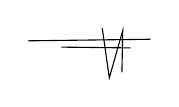
\begin{tikzpicture}[x=1cm,y=1cm]
\draw (0,0)--(1.55,.02);\draw (.42,-.08)--(1.3,-.09);\draw (.94,.16)--(1.03,-.47)--(1.2,.13)--(1.19,-.4);
\end{tikzpicture}}

\uline{Preuve prop. 3} \inserted{On peut supposer $S$ affine.} De $1^\circ)$ résulte que l'ens \deleted{de} $M(T,\eta)$ est stable par \deleted{\unsure{double}} générisation. Par $2^\circ)$, il est donc ouvert. \deleted{Donc pour $\forall$ \unsure{d'où le}} \inserted{Utilisant $\underset{\leftarrow}{L}_2$,} Pour $\forall a\in S$ et $x\in X_a$ sur $a$, \deleted{\unsure{soit}} il existe donc un \unsure{«} $X^{(*)}$ \deleted{\unsure{local}} affine, \deleted{loc.} de t. fini sur $S$, et $\eta^{(*)}\in F(X^{(*)})$, \uline{modulaire} \inserted{local} en
\mspage{36}
\scanpage{38}
\begin{center}$-\ 27\ -$\end{center}
\hfill n$^\circ$ 371

tion ainsi définie sur $A^S$ est $A$-bilinéaire et vérifie les relations (5) du n$^\circ$ 1 ; en outre, elle est \uline{associative}, car on a
\[
\sum_{uvw=t}\alpha_u\beta_v\gamma_w=\sum_{rw=t}\left(\left(\sum_{uv=r}\alpha_u\beta_v\right)\gamma_w\right)=\sum_{us=t}\left(\alpha_u\left(\sum_{vw=s}\beta_v\gamma_w\right)\right).
\]
Cette multiplication et la structure de $A$-module de $A^S$ \unsure{définissent|définissant} donc sur $A^S$ une structure d'\uline{algèbre associative} par rapport à $A$ ; nous dirons que l'ensemble $A^S$, muni de cette structure, est l'\uline{algèbre large du monoïde} $S$, relative à l'anneau $A$.

Il est immédiat que l'\uline{algèbre} $A^{(S)}$ du monoïde $S$ relative à $A$ (dite encore \uline{algèbre stricte} de $S$ lorsqu'on veut éviter toute confusion) est une \uline{sous-algèbre} de l'algèbre large de $S$ relative à $A$ (et est identique à cette dernière lorsque $S$ est fini). \uline{Par abus de langage}, on note encore tout élément $(\xi_s)_{s\in S}$ de l'algèbre large de $S$ relative à $A$ par la même notation $\sum_{s\in S}\xi_s s$ que les éléments de l'algèbre stricte de $S$ ; bien entendu le signe de sommation qui figure dans cette notation ne représente aucune opération algébrique puisqu'il porte sur une \uline{infinité} de termes $\ne0$. Avec cette notation, la multiplication dans l'algèbre large de $S$ est encore donnée par la formule (23) du n$^\circ$ 11.

Si $S$ est commutatif, il en est de même de son algèbre large $A^S$ ; si $S$ admet un élément neutre $u$, $u$ est aussi élément unité de $A^S$. Si $T$ est une partie stable de $S$, l'algèbre large $A^T$ du monoïde $T$ s'identifie canoniquement à une sous-algèbre de l'algèbre large de $S$.

Parmi les monoïdes satisfaisant à la condition (D), citons en particulier l'ensemble $N$ des entiers naturels, muni de la structure définie par l'\uline{addition}, et l'ensemble $N^*$ des entiers $\ge1$, muni de la structure définie par la \uline{multiplication}. Au chap. IV, nous étudierons l'algèbre stricte (anneau des polynômes sur $A$ à une indéterminée) et l'algèbre
\mspage{37}
\scanpage{39}
tous les pts de $X^{(*)}$.

\deleted{Pour \unsure{les}}
\deleted{Tout \unsure{On veut donc} que les $X^{(a)}$ se recollent \unsure{$(X,\eta)$ correspondants}: $\forall$ couple $(a,b)$, soit $X^{(a,b)}$ l'ens des $u\in\unsure{X^{a,a}|X^{(a)}}$ qui sont \unsure{apparentés} à un pt de $X^b$. D'après ce qui précède \inserted{et $\underset{\leftarrow}{L}_2$ \unsure{il résulte} que c'est} \unsure{on a} un ens \uline{ouvert}. De plus, on a un}

\uline{Lemme} Soit $(Z,\eta)$ ($Z$ loc. de t. fini sur $S$, $\eta\in F(\unsure{S|Z})$) tel que pour $\forall z\in Z$, $\eta_z$ soit modulaire. Considérons $h_Z\xrightarrow{\eta}F$, \deleted{et}
Alors $h_Z\times_F h_Z\subset h_{Z\times Z}$ est représentable par un sous-préschéma de $Z\times Z$, soit $Z'$. Les projections
\diagram{\begin{tikzcd}
Z'\arrow[r,shift left=.6ex,"p_1"]\arrow[r,shift right=.6ex,"p_2"']&Z
\end{tikzcd}}
sont des isomorphismes locaux, [et font de $Z'$ un \deleted{préschéma} graphe d'équivalence dans $Z$ \unsure{$\ldots$}].
\margin{Reprendre les conditions \inserted{nécessaires} sur $F$. Elles sont: \unsure{bien plus faibles}\ldots}

\unsure{AQT}
Or sous les conditions précédentes, prenant $Z=X^{(*)}$, on voit que quand on se restreint au dessus de $S_a$, alors
\diagram{\begin{tikzcd}
Z'_a\arrow[r,shift left=.6ex]\arrow[r,shift right=.6ex]&Z_a
\end{tikzcd}}
est la relation d'équivalence \uline{triviale}. Donc
\mspage{38}
\scanpage{40}
\begin{center}-- 26 -- \hfill n° 371\end{center}
qu'il existe un homomorphisme unique de monoïdes $\varphi:L(S)\to B$ (chap. I, \uline{Rectifications} au fasc. IV) tel que $\varphi(e)=1$, $\varphi(\alpha)=\alpha$ pour tout $\alpha\in S$; par suite, si $A$ est l'algèbre du monoïde $L(S)$ par rapport à $Z$, il y a un homomorphisme unique d'anneaux $\bar\varphi:A\to B$ tel que $\bar\varphi(e)=1$ et $\bar\varphi(\alpha)=\alpha$ pour tout $\alpha\in S$. \uline{Supposons} que la relation $\bar\varphi(\lambda)=0$ implique $\lambda.x=0$ pour tout $x\in M$; autrement dit le noyau $n$ de $\bar\varphi$ est contenu dans l'annulateur de $A$-module $M$; on satisfait donc encore aux conditions 1) et 2) en considérant sur $M$ la structure de $(A/n)$-module associée à sa structure de $A$-module (chap. II, 3\textsuperscript{e} éd., § 12), et on notera que dans ce cas $A/n$ s'identifie au \uline{sous-anneau} de $B$ \uline{engendré par} $S$.

12. \uline{Exemples d'algèbres} : VI. \uline{Algèbre large d'un monoïde}.

L'algèbre d'un monoïde $S$ relative à un anneau commutatif $A$ est (en tant que $A$-module) le sous-module du produit $A^S$ formé des familles $(\alpha_s)_{s\in S}$ de support fini; la multiplication dans cette algèbre est définie par la relation $(\alpha_s)(\beta_s)=(\gamma_s)$ où, pour tout $s\in S$
\[
(25)\qquad \gamma_s=\sum_{tu=s}\alpha_t\beta_u.
\]
La somme du second membre de (25) a un sens parce que $(\alpha_s)$ et $(\beta_s)$ sont des familles de support fini, et il en est donc de même de la famille double $(\alpha_t\beta_u)_{(t,u)\in S\times S}$. Mais le second membre de (25) a encore un sens pour des éléments \uline{quelconques} $(\alpha_s)$, $(\beta_s)$ de $A^S$ lorsque le monoïde $S$ satisfait à la condition suivante :

(D) \uline{Pour tout} $s\in S$, \uline{il n'existe qu'un nombre fini de couples} $(t,u)$ \uline{d'éléments de} $S$ \uline{tels que} $tu=s$.

Supposons donc que $S$ vérifie la condition (D); sur le $A$-module produit $A^S$, on peut alors définir une loi de composition interne $((\alpha_s),(\beta_s))\to(\gamma_s)$ où, pour tout $s\in S$, $\gamma_s$ est donné par la formule (25). Il est immédiat que la multiplica-
\mspage{39}
\scanpage{41}
il en est de même de $Z'|U=Z|U$, si $U$ est un voisinage ouvert convenable de $a$. En d'autres termes, \uline{à condition de prendre $\unsure{X^{(*)}|X^{(x)}}$ assez petit}, on peut supposer que $(X^{(x)},\unsure{\eta^{(x)}|\xi^{(x)}})$ est ``\inserted{quasi-}\uline{modulaire}'' [Préciser la signification de ce terme : \inserted{$\unsure{\eta_x|y_x}:h_{X^{(x)}}\to F$ est une immersion ouverte}]. Alors, une autre proposition ``formelle'' nous permet de recoller les $X^{(x)}$ et de trouver un $(X,\xi)$ qui représente $F$. (grâce à $L_2$).
\mspage{40}
\scanpage{42}
\begin{center}-- 25 -- \hfill n° 371\end{center}
lois externes sur $M$. Soit $\Omega$ l'ensemble \uline{somme} (\uline{Ens.}, chap. II, § 4, n° 8) des domaines d'opérateurs des diverses lois externes de $M$, chacun de ces domaines d'opérateurs étant identifié canoniquement à la partie de $\Omega$ qui lui correspond. Soit $L(\Omega)$ le \uline{monoïde libre} (chap. I, 3\textsuperscript{e} éd., § 1, n° 3) déduit de $\Omega$; nous définirons une loi de composition externe $(\alpha,x)\to\alpha x$ sur $M$, ayant $L(\Omega)$ comme domaine d'opérateurs, par récurrence sur la longueur du \uline{mot} $\alpha$ dans $L(\Omega)$; si $\alpha$ est de longueur $0$, c'est le mot vide $e$, et nous posons $ex=x$ pour tout $x\in M$. Si maintenant $\alpha$ est de longueur $n\geq1$, on peut l'écrire d'une seule manière sous la forme $\alpha=\beta\gamma$, où $\gamma$ est de longueur $n-1$ et $\beta$ de longueur $1$; $\beta$ appartient par suite à un et un seul des domaines d'opérateurs des lois externes données sur $M$ et $\beta y$ est donc défini pour tout $y\in M$; on pose alors $\alpha x=\beta(\gamma x)$. Pour deux mots quelconques $\alpha$, $\beta$ dans $L(\Omega)$, on vérifie que l'on a $\alpha(\beta x)=(\alpha\beta)x$ pour tout $x\in M$, par récurrence sur la longueur de $\alpha$.

Soit maintenant $A$ l'algèbre du monoïde $L(\Omega)$ relative à l'anneau $Z$ des entiers rationnels; on définit une loi externe $(\alpha,x)\to\alpha x$ sur $M$, ayant $A$ pour anneau d'opérateurs, en posant, pour tout $\alpha=\sum_{\lambda\in L(\Omega)}n_\lambda.\lambda$ (avec $n_\lambda\in Z$ et $n_\lambda=0$ sauf pour un nombre fini de valeurs de $\lambda$),
\[
\alpha x=\sum_{\lambda\in L(\Omega)}n_\lambda(\lambda x).
\]
On vérifie sans peine que cette loi externe satisfait aux axiomes $(\unsure{M_{\mathrm I}|N_{\mathrm I}})$, $(M_{\mathrm{II}})$, $(M_{\mathrm{III}})$ et $(M_{\mathrm{IV}})$ du chap. II, 3\textsuperscript{e} éd., § 1, n° 1; elle définit donc sur $M$ une structure de $A$-module à gauche, et il est immédiat que cette structure satisfait aux conditions 1) et 2) ci-dessus.

La méthode précédente s'applique à des groupes commutatifs à opérateurs quelconques; mais si on ne considère que des groupes commutatifs dont les opérateurs satisfont à certaines conditions supplémentaires, on peut souvent satisfaire aux conditions 1) et 2) en associant d'une autre manière une structure de module à la structure donnée de groupe à opérateurs sur $M$.

Par exemple, supposons qu'il n'y ait sur $M$ qu'une seule loi externe, dont le domaine d'opérateurs soit \uline{une partie} $S$ \uline{d'un anneau} $B$; on sait
\mspage{41}
